\documentclass{article}
\title{CSCI 2200 HW1}
\author{Xinshi,Wang}
\usepackage[letterpaper,textwidth=5.5in,right=0.6in,textheight=9in,left=0.6in,top=0.7in,bottom=0.7in]{geometry}
\usepackage{scrextend}
\usepackage{graphicx}
\usepackage{xcolor}
\usepackage{amssymb}
\usepackage{amsmath}
\usepackage{setspace}
\usepackage{mathrsfs}
\usepackage[utf8]{inputenc}
\usepackage{mathtools}
\usepackage{tikz}
\begin{document}
\noindent
CSCI 2200 HW9\\
Wang Xinshi\\

%Q 13.51 starts from here
\begin{addmargin}[2em]{2em}
	\text{\bf Problem 22.14.} Answer true or false.\\
	(a) A bijection must be an injection.\\
	(b) There is a bijection from Q to R.\\
	(c) There is a bijection from Q to Z.\\
	(d) There is an uncountable subset of N × N.\\
	(e) Every infinite subset of R is uncountable.\\
	(f) The solutions to $x \equiv 0$ (mod 6) are countable.\\\\
	(a). True. A function that is bijective is both injective and surjective.\\
	(b). False. The set $\mathbb{Q}$ is countable and the set $\mathbb{R}$ is an infinite set. Thus they have different cardinalites. Thus there does not exist a bijection from $\mathbb{Q}$ to $\mathbb{R}$.\\
	(c).True. The set $\mathbb{Q}$ and the set $\mathbb{Z}$ have the same cardinality which is $\aleph_0$. Thus there exists a bijection from $\mathbb{Q}$ to $\mathbb{Z}$.\\
	(d).False. The set $\mathbb{N} \times \mathbb{N}$ is countable since it is the cartesian product of a countable set.\\
	(e).False, the natural number as a infinite subset of $\mathbb{R}$ is denumerable and infinite, which means it is also countable.\\
	(f).True.  $x \equiv 0$ (mod 6) is a subset of $\mathbb{N}$. Since it is a subset of a countable set, it is countable.
\end{addmargin}
%Q 11.13 ends here
\clearpage


\begin{addmargin}[2em]{2em}
	\text{\bf Problem 23.30}. Find regular expressions for $\mathcal{L}$ and its reversal $\mathcal{L}$ (Problem 23.24), where strings of $\mathcal{L}$ satisfy: Every 0 is followed by at least one 1.\\
	$\mathcal{L} = \{\omega|\text{Every 0 is followed by at least one 1}\} = \{\{1\}^* \cdot \{0\} \cdot \{1\} \cdot \{1\}^* \}^*$\\
	The reversal of the regular expression is every $0$ is followed by no $1$.\\
	$\mathcal{L} = \{\omega|\text{Every 1 is followed by }\} =  \{\{1\}^* \cdot \{1\} \cdot \{0\} \cdot \{1\}^* \}^* $\\
\end{addmargin}

%Q 12.74(k) ends here
\clearpage

\begin{addmargin}[2em]{2em}
	\text{\bf Problem 24.3.}  Describe in words the language accepted by each automaton, and also give a regular expression..\\
	\begin{figure}[h]
		\begin{center}
			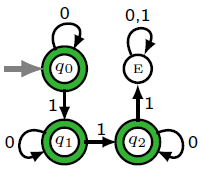
\includegraphics[scale = 0.6]{"C:/Users/Micha/OneDrive - Rensselaer Polytechnic Institute/CSCI 2200/Latex_pictures/24_03a.png"}\\
		\end{center}
	\end{figure}
	
	The Automata represents the language $\mathcal{L}=\{\omega|\text{There cannot be more than two 1s}\}$. The regular expression for the Automata is $\{0\}^* \cdot \{1\} \cdot \{0\}^* \cdot \{1\} \cdot \{0\}^* \cup \{0\}^* \cdot \{1\} \cdot \{0\}^* \cup \{0\}^*$.
\end{addmargin}
\clearpage
\begin{addmargin}[2em]{2em}
	\text{\bf Problem 24.10.} A voomba vacuum-rover $\triangle$, when placed on one end of a dirt path, should move step
		by step and vacuum up all the dirt. The voomba can sense dirt in the square ahead, can rotate 90° clockwise,
		can move forward and transition among its internal states. Design a voomba as a DFA. In the picture, the
		voomba is facing north, left of the first piece of dirt.
		When will your voomba succesfully vacuum all the dirt? Give an informal argument.\\
		\begin{figure}[h]
			\begin{center}
				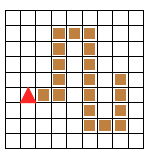
\includegraphics[scale = 0.6]{"C:/Users/Micha/OneDrive - Rensselaer Polytechnic Institute/CSCI 2200/Latex_pictures/cleaner.png"}\\
			\end{center}
		\end{figure}
	
	\text{\bf Answer}\\
\begin{center}
	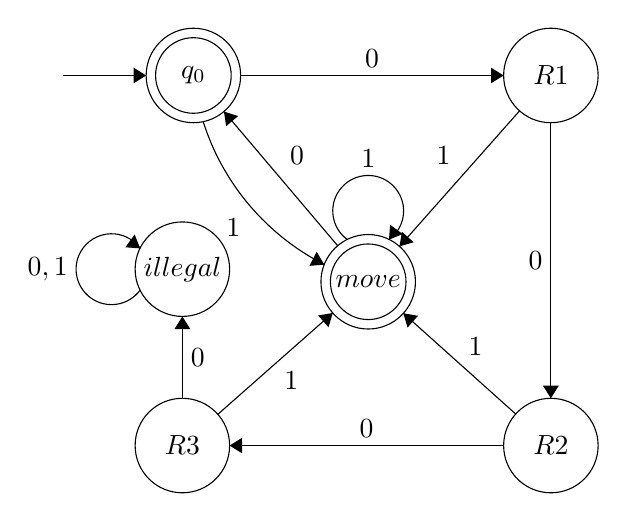
\begin{tikzpicture}[scale=0.2]
		\tikzstyle{every node}+=[inner sep=0pt]
		\draw [black] (16.8,-12.1) circle (3);
		\draw (16.8,-12.1) node {$q_0$};
		\draw [black] (16.8,-12.1) circle (2.4);
		\draw [black] (39.5,-12.1) circle (3);
		\draw (39.5,-12.1) node {$R1$};
		\draw [black] (39.5,-35.6) circle (3);
		\draw (39.5,-35.6) node {$R2$};
		\draw [black] (16.1,-35.6) circle (3);
		\draw (16.1,-35.6) node {$R3$};
		\draw [black] (27.9,-25.2) circle (3);
		\draw (27.9,-25.2) node {$move$};
		\draw [black] (27.9,-25.2) circle (2.4);
		\draw [black] (16.1,-24.4) circle (3);
		\draw (16.1,-24.4) node {$illegal$};
		\draw [black] (19.8,-12.1) -- (36.5,-12.1);
		\fill [black] (36.5,-12.1) -- (35.7,-11.6) -- (35.7,-12.6);
		\draw (28.15,-11.6) node [above] {$0$};
		\draw [black] (8.5,-12.1) -- (13.8,-12.1);
		\fill [black] (13.8,-12.1) -- (13,-11.6) -- (13,-12.6);
		\draw [black] (39.5,-15.1) -- (39.5,-32.6);
		\fill [black] (39.5,-32.6) -- (40,-31.8) -- (39,-31.8);
		\draw (39,-23.85) node [left] {$0$};
		\draw [black] (36.5,-35.6) -- (19.1,-35.6);
		\fill [black] (19.1,-35.6) -- (19.9,-36.1) -- (19.9,-35.1);
		\draw (27.8,-35.1) node [above] {$0$};
		\draw [black] (18.35,-33.62) -- (25.65,-27.18);
		\fill [black] (25.65,-27.18) -- (24.72,-27.34) -- (25.38,-28.09);
		\draw (23.01,-30.89) node [below] {$1$};
		\draw [black] (25.112,-24.105) arc (-117.01247:-162.43643:15.405);
		\fill [black] (25.11,-24.11) -- (24.63,-23.3) -- (24.17,-24.19);
		\draw (19.81,-21.78) node [left] {$1$};
		\draw [black] (25.96,-22.91) -- (18.74,-14.39);
		\fill [black] (18.74,-14.39) -- (18.88,-15.32) -- (19.64,-14.68);
		\draw (22.9,-17.21) node [right] {$0$};
		\draw [black] (37.51,-14.35) -- (29.89,-22.95);
		\fill [black] (29.89,-22.95) -- (30.79,-22.69) -- (30.04,-22.02);
		\draw (33.16,-17.2) node [left] {$1$};
		\draw [black] (26.577,-22.52) arc (234:-54:2.25);
		\draw (27.9,-17.95) node [above] {$1$};
		\fill [black] (29.22,-22.52) -- (30.1,-22.17) -- (29.29,-21.58);
		\draw [black] (37.27,-33.6) -- (30.13,-27.2);
		\fill [black] (30.13,-27.2) -- (30.4,-28.11) -- (31.06,-27.36);
		\draw (34.71,-29.91) node [above] {$1$};
		\draw [black] (16.1,-32.6) -- (16.1,-27.4);
		\fill [black] (16.1,-27.4) -- (15.6,-28.2) -- (16.6,-28.2);
		\draw (16.6,-30) node [right] {$0$};
		\draw [black] (13.42,-25.723) arc (-36:-324:2.25);
		\draw (8.85,-24.4) node [left] {$0,1$};
		\fill [black] (13.42,-23.08) -- (13.07,-22.2) -- (12.48,-23.01);
	\end{tikzpicture}
\end{center}

	Consider each square of the grid as either 0(has no dirt) or 1(has dirt). Thus we have a 2-dimensional list that represents the map. $R_1$,$R_2$, and $R_3$ each represents a rotation, which rotates the reading head 90° if the bit pointed by the reading head is a 0, but will not process the next bit. After it detects a 1 bit, it transits to the move state and process the next bit. If the next bit is still a one, continue cleaning; otherwise return to the $q_0$ state and rotate to find the next direction. If after 3 roatation it still could not find a direction, it means there are no more dirts sorrounding, and turn into illegal state. It will eventually bump into the wall and terminate. It can clean up all the dirts if the dirt path is continuous.
\end{addmargin}
\clearpage
\begin{addmargin}[2em]{2em}
	\text{\bf Problem 24.50.} Find a DFA to solve each problem, or prove that no such DFA exists. Strings with 3 times as many 0’s as 1’s.\\\\
	The problem is $\mathcal{L} = \{0^{3n}1^n|n \in \mathbb{N}\}$
	Assume such DFA exists and can be solved with k states. Consider binary string $S = 00...0$(k 0s). Thus we have the following transition $q_0 \rightarrow state(0) \rightarrow state(0^2) \rightarrow state(0^3) \rightarrow ... \rightarrow state(0^k)$. Thus we have visited $k+1$ states. By the pigenhole theorem, there must have 3i and 3j with $3i \neq 3j$ such that state($0^{3i}$) = state($0^{3j}$) = q. Thus we have $q|0^{3i} \triangleright 1^i$ and $q|0^{3j} \triangleright 1^i$ produces the same result. However, since $3j \neq 3i$, we found a contradiction. Thus there does not exist such automata.
\end{addmargin}
\end{document}